\section{Introduction}

\begin{frame}{Skills in manipulation and locomotion\\ are needed}
\begin{center}
  \vspace*{0.7cm}
  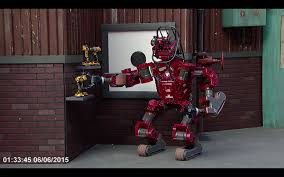
\includegraphics[height=3cm]{darpa/drill.jpeg}
  \hspace*{0.5cm}
  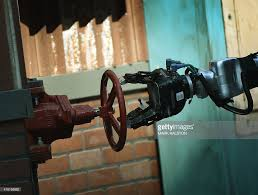
\includegraphics[height=3cm]{darpa/valve.jpeg}\\[0.2cm]
  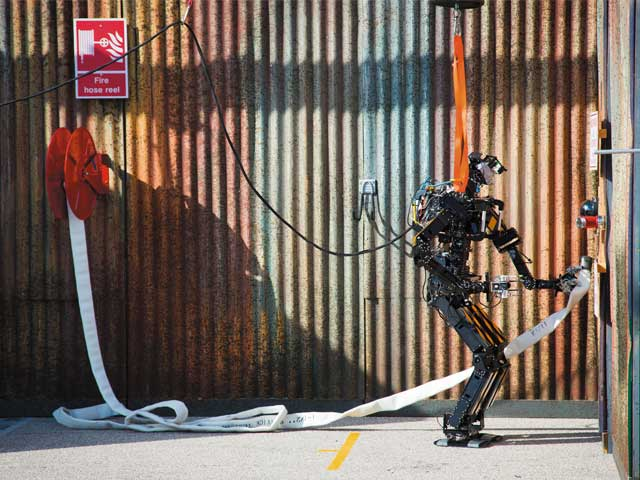
\includegraphics[height=3cm]{darpa/hose.jpg}
\end{center}
%\begin{itemize}
%  \item 
%\end{itemize}
\end{frame}


\begin{frame}{Problem}{Problem presentation}

\begin{equation}
  \label{eq:equilibrium_constraints}
  m
  \begin{bmatrix}
  \ddcom - {\bf g} \\
  \com \times (\ddcom - {\bf g})
  \end{bmatrix}
  +
  \begin{bmatrix}
  {\bf 0} \\
  \dot{\mathcal{L}}
  \end{bmatrix}
  =
  \begin{bmatrix}
  \sum_{i=1}^{M}
  \Qf \ff \\
  \sum_{i=1}^{M}
  \pf \times \Qf  \ff
\end{bmatrix}
\end{equation}


\end{frame}